\documentclass[12pt, a4paper, oneside]{ctexart}
\usepackage{amsmath, amsthm, amssymb, bm, color, graphicx, geometry, mathrsfs,extarrows, braket, booktabs, array}
\usepackage[colorlinks,linkcolor=red,anchorcolor=blue,citecolor=green]{hyperref}

\linespread{1.4}
%\geometry{left=2.54cm,right=2.54cm,top=3.18cm,bottom=3.18cm}
\geometry{left=1.84cm,right=1.84cm,top=2.18cm,bottom=2.18cm}
\newenvironment{problem}{\par\noindent\textbf{题目. }}{\bigskip\par}
\newenvironment{solution}{\par\noindent\textbf{解答. }}{\bigskip\par}
\newenvironment{note}{\par\noindent\textbf{注记. }}{\bigskip\par}

\everymath{\displaystyle} % 默认全部行间公式
\DeclareMathOperator*\lowlim{\underline{lim}} % lower limits
\DeclareMathOperator*\uplim{\overline{lim}} % upper limits
\let\leq=\leqslant % 将全部leq变为leqslant
\let\geq=\geqslant % geq同理

% 一些宏定义
\def\bd{\boldsymbol}    % 加粗(向量) boldsymbol
\def\disp{\displaystyle}% 使用行间公式 displaystyle(默认)
\def\tsty{\textstyle}   % 使用行内公式 textstyle
\def\sign{\text{sign}}  % sign function
\def\wtd{\widetilde}    % 宽波浪线 widetilde
\def\R{\mathbb{R}}      % Real number
\def\C{\mathbb{C}}      % Complex number
\def\d{\mathrm{d}}      % differential operator
\def\e{\mathrm{e}}      % Euler's number
\def\i{\mathrm{i}}      % imaginary number
\def\re{\mathrm{Re}\,}    % Real part
\def\im{\mathrm{Im}\,}    % Imaginary part
\def\L{\mathcal{L}}     % Loss function
\def\wdh{\widehat}      % 宽帽子 widehat
\def\ol{\overline}      % 上横线 overline
\def\ul{\underline}     % 下横线 underline
\def\add{\vspace{1ex}}  % 增加行间距
\def\del{\vspace{-3.5ex}}  % 减少行间距

% 基本信息
\newcommand{\RQ}{\today} % 日期
\newcommand{\km}{复变函数} % 科目
\newcommand{\bj}{强基数学002} % 班级
\newcommand{\xm}{吴天阳} % 姓名
\newcommand{\xh}{2204210460} % 学号

\begin{document}

%\pagestyle{empty}
\pagestyle{plain}
\vspace*{-15ex}
\centerline{\begin{tabular}{*5{c}}
    \parbox[t]{0.25\linewidth}{\begin{center}\textbf{日期}\\ \large \textcolor{blue}{\RQ}\end{center}} 
    & \parbox[t]{0.2\linewidth}{\begin{center}\textbf{科目}\\ \large \textcolor{blue}{\km}\end{center}}
    & \parbox[t]{0.2\linewidth}{\begin{center}\textbf{班级}\\ \large \textcolor{blue}{\bj}\end{center}}
    & \parbox[t]{0.1\linewidth}{\begin{center}\textbf{姓名}\\ \large \textcolor{blue}{\xm}\end{center}}
    & \parbox[t]{0.15\linewidth}{\begin{center}\textbf{学号}\\ \large \textcolor{blue}{\xh}\end{center}} \\ \hline
\end{tabular}}
\vspace*{4ex}

% 正文部分
\paragraph{第五章}\del

\paragraph{2.}求下列级数的收敛范围:
\begin{equation*}
    (1)\ \sum_{n=1}^\infty\frac{\cos nz}{n^2};\qquad(2)\ \sum_{n=1}^\infty\frac{z^n}{1-z^n}.
\end{equation*}
\begin{solution}
    (1) 当$z\in \mathbb{R}$时, 设$0 < \delta < \pi,\ \forall x \in [\delta, 2\pi - \delta]$, 则有
    \begin{equation*}
        \sum_{k=1}^ne^{ikx} = \left|\frac{e^{ix}(1-e^{inx})}{1-e^{ix}}\right| \leqslant \frac{2}{|1-e^{ix}|} = \frac{2}{|e^{i\frac{x}{2}}-e^{-i\frac{x}{2}}|} = \frac{1}{|\sin\frac{x}{2}|}\leqslant \frac{1}{|\sin\frac{\delta}{2}|},
    \end{equation*}
    由于$\frac{1}{n^2}$单调趋于$0$, 由Dirichlet判别法知, $ \sum_{n=1}^\infty\frac{\cos nx}{n^2}$收敛.

    当$z\in \C-\R$时, 令$z = iy$, 当$n\rightarrow \infty$时, 通项$ \frac{\cos nz}{n^2}=\frac{e^{-ny}+e^{ny}}{n^2}\rightarrow \infty$, 所以级数发散.

    综上, 该级数的收敛范围为$\R$.

    (2) 由于级数收敛的充分条件为通项趋于$0$, $ \frac{z^n}{1-z^n} = 1-\frac{1}{1-z^n} \rightarrow 0\Rightarrow z^n\rightarrow 0\Rightarrow |z| < 1$, 又由于当$|z|<1$时, 有
    \begin{equation*}
        \sum_{k=n+1}^{n+p}\frac{z^n}{1-z^n} = n+p-\frac{1}{1-z^n+1}-\cdots-\frac{1}{1-z^{n+p}}\leqslant n+p-\frac{n+p}{1-z^n} = (n+p)(1-\frac{1}{1-z^n})\rightarrow 0.
    \end{equation*}

    所以该级数的收敛范围为$|z|<1$.
\end{solution}
\paragraph{3.}证明: 级数$ \sum_{n=1}^\infty(-1)^n\left(\frac{1}{z-n}+\frac{1}{n}\right)$在不包含正整数的任意有界闭集上一致收敛.
\begin{proof}
    令$K$为$\C$中满足题意的任意紧集, 则存在$R\in\R$使得$|z|<R$包住$K$, 取$N > R$, 于是$\forall n > N$, 有
    \begin{equation*}
        \left|(-1)^n\left(\frac{1}{z-n}+\frac{1}{n}\right)\right| = \left|\frac{z}{n(z-n)}\right|\leqslant \frac{M}{n^2-Mn}=\frac{1}{n-M}-\frac{1}{n},
    \end{equation*}
    其中$ M = \left[\sup_{z\in K}|z|\right]+1$, 上式中不等号的原因是
    \begin{equation*}
        |z-n|\geq n-\re z\geq n-M.   
    \end{equation*}
    
    由于级数$\sum_{k=M+1}^n\left(\frac{1}{k-M}-\frac{1}{k}\right) = \sum_{k=1}^M\frac{1}{k}-\sum_{k=n-m+1}^n\frac{1}{k}$, 当$n\rightarrow \infty$时,\add 极限存在, 由M-判别法可知, 级数在$K$上一致收敛.
\end{proof}
\paragraph{4.}证明: 级数$ \sum_{n=1}^\infty\frac{(-1)^{n-1}}{z+n}$在不包含负整数的任意有界闭集上一致收敛.
\begin{proof}
    令$K$为$\C$中满足题意的任意紧集, 则存在充分大的$N$使得$N > |z|+1,\ (z\in K)$, 不妨令$N$为奇数, 对于任意$n>N$, 由于
    \begin{align}
        \nonumber\left|\sum_{k=N}^{2n}\frac{(-1)^{k-1}}{z+k}\right| \leq&\ \left|\frac{1}{z+N}-\frac{1}{z+N+1}\right|+\cdots+\left|\frac{1}{z+2n-1}-\frac{1}{z+2n}\right|\\
        \nonumber=&\ \left|\frac{1}{(z+N)(z+N+1)}\right|+\cdots+\left|\frac{1}{(z+2n-1)(z+2n)}\right|\\
        \nonumber=&\ \frac{1}{|z+N||z+N+1|}+\cdots+\frac{1}{|z+2n-1||z+2n|}\\
        \label{eq-估计}\leq&\ \frac{1}{N'\cdot (N'+1)}+\cdots+\frac{1}{(2n-1)(2n)}\\
        \nonumber=&\ \frac{1}{N'}-\frac{1}{N'+1}+\cdots+\frac{1}{2n-1}-\frac{1}{2n}\\
        \nonumber=&\ \sum_{n=N'}^{2n}\frac{(-1)^{n-1}}{n}\rightarrow 0,\quad(N'\to \infty)
    \end{align}
    其中$N' = [N-|z|] $, $[\cdot ]$表示向下取整, 由于$N>|z|+1$, 则$N' \geq 1$. (\ref{eq-估计})式的不等号是因为
    \begin{equation*}
        |z+N+k|\geq \re z + N +k\geq N-|z| + k\geq [N-|z|] + k= N'+k.
    \end{equation*}

    由Leibniz判别法可知$\sum_{n=1}^\infty\frac{(-1)^{n-1}}{n}$收敛, 所以上式最后一项当$N\to\infty$时, 有 $N'\to\infty$该数项级数趋于$0$, 由Cauchy收敛原理知$S_{2n}$一致收敛, 又由于$S_{2n+1}\leqslant S_{2n}+ \frac{1}{|z+2n+1|}$, 同理可证$S_{2n+1}$一致收敛. 综上, 级数在$K$上一致收敛.
\end{proof}
\paragraph{6.}设幂级数$ \sum_{n=0}^\infty c_nz^n$的收敛半径$R > 0$, 和函数为$f(z)$. 证明: 当$0 < r < R$时, 

(1) $ \frac{1}{2\pi}\int_0^{2\pi}|f(r\e^{i\theta})|^2\,\d\theta = \sum_{n=0}^\infty|c_n|^2r^{2n};$

(2) 若$f(z)$在圆$|z| < R$内有界, 可设为$|f(z)|\leqslant M$, 则$ \sum_{n=0}^\infty|c_n|^2R^{2n}\leqslant M^2.$

\begin{proof}
    (1) 
    \begin{equation*}
        \frac{1}{2\pi}\int_0^{2\pi}|f(re^{i\theta})|^2\,\d\theta = \frac{1}{2\pi}\int_0^{2\pi}\left|\sum_{n=0}^{\infty}c_nr\e^{in\theta}\right|^2\,\d\theta = \frac{1}{2\pi}\int_0^{2\pi}\left(\sum_{n=0}^{\infty}c_nr^n\e^{in\theta}\right)\left(\sum_{m=0}^{\infty}\bar{c}_mr^m\e^{-im\theta}\right)\,\d\theta,
    \end{equation*}
    由于$ \sum_{n=0}^\infty c_nr^n\e^{in\theta},\ \sum_{m=0}^\infty \bar{c}_mr^m\e^{-im\theta}$在圆$|z|\leqslant r$内均一致收敛, 则两级数之积也一致收敛, 则可逐项积分, 当$n\neq m$时, 有
    \begin{equation*}
        \frac{1}{2\pi}\int_0^{2\pi}c_n\bar{c}_mr^{n+m}\e^{i(n-m)\theta}\,\d\theta = \frac{c_n\bar{c}_mr^{n+1}}{2\pi i(n-m)}\e^{i(n-m)\theta}\biggl|_0^{2\pi} = 0,
    \end{equation*}
    所以
    \begin{equation*}
        \frac{1}{2\pi}\int_0^{2\pi}|f(re^{i\theta})|^2\,\d\theta = \sum_{n=0}^{\infty}\frac{1}{2\pi}\int_0^{2\pi}c_n\bar{c}_nr^{2n}\,\d\theta = \sum_{n=0}^\infty|c_n|^2r^{2n}.
    \end{equation*}

    (2) 由(1)可得$ \sum_{n=0}^\infty|c_n|^2r^{2n}=\frac{1}{2\pi}\int_0^{2\pi}|f(r\e^{i\theta})|^2\,\d\theta\leqslant \frac{1}{2\pi}\int_0^{2\pi}M^2\,\d\theta = M^2$, 令$r\to R$得证.
\end{proof}
\paragraph{7.}若幂级数$ \sum_{n=0}^\infty c_nz^n$在单位元$|z|<1$内收敛到有界函数$f(z)$, 证明$ \lim_{n\to\infty}c_n=0$.
\begin{proof}
    由6.(2)可知, 令$|f(z)|\leqslant M$, 则$\sum_{n=0}^\infty|c_n|^2\leqslant M^2$, 由于收敛级数通项恒正, 所以通项趋于$0$, 即$\lim_{n\to \infty}c_n=0$.
\end{proof}
\paragraph{8.}设$ \sum_{n=0}^\infty c_nz^n$在$|z|\leqslant R$上收敛$(0 < R < +\infty)$, 求证$\varphi(z) = \sum_{n=0}^\infty\frac{c_n}{n!}z^n$在$\C$上解析, 且$|\varphi(z)|\leqslant M\e^{|z|/R}$.
\begin{proof}
    由收敛半径计算公式知$\uplim_{n\to\infty}\sqrt[n]{|c_n|} = \frac{1}{R}$, 则$\uplim_{n\to\infty}\sqrt[n]{\frac{|c_n|}{n!}} = 0$, 因此$\sum_0^{\infty}\frac{c_n}{n!}z^n$的收敛半径为$+\infty$, 所以$\varphi(z)$在$\C$上解析. 由于$\sum_{n=0}^\infty c_nz^n$收敛, 则一般项趋于$0$, 存在$M > 0$使得$|c_nz^n|\leqslant M$, 令$z\to R$, 得$|c_n|R^n\leqslant M$, 则
    \begin{equation*}
        |\varphi(z)| = \left|\sum_{n=0}^\infty \frac{c_n}{n!}z^n\right|\leqslant \sum_{n=0}^\infty \frac{|c_n|}{n!}|z|^n\leqslant \sum_{n=0}^\infty \frac{|c_n|R^n}{n!}\,\frac{|z|^n}{R^n}\leqslant M\sum_{n=0}^\infty\frac{1}{n!}\,\frac{|z|^n}{R^n} = M\e^{|z|/R}.
    \end{equation*}
\end{proof}
\del
\paragraph{9.}证明: (1) 对任意的复数$z$, $|\e^z-1|\leq \e^{|z|}-1\leq |z|e^{|z|};$\add

(2) 当$0<|z|<1$时, $\frac{1}{4}|z|<|\e^z-1|<\frac{7}{4}|z|.$
\begin{proof}
    (1)\del
    \begin{align*}
        |\e^z-1| = \left|\sum_{n=1}^\infty\frac{z^n}{n!}\right|\leq \sum_{n=1}^\infty\frac{|z|^n}{n!} = \e^{|z|}-1\leq&\ (1+|z|)(e^{|z|}-1) = (1+|z|)\e^{|z|}-|z|-1\\
        \leq&\ (1+|z|)\e^{|z|}-\e^{|z|}=|z|\e^{|z|}.
    \end{align*}
    \del

    (2) 由最大模原理可知, $\left|\frac{e^z-1}{z}\right|$的最大值在$|z| = 0$或$|z|=1$上取到, 当$|z|=0$时, $\left|\frac{e^z-1}{z}\right| = |e^z| = 1$, 满足题意.\add

    当$|z| = 1$时, 
    \begin{align*}
        \max_{|z| = 1}\left|\frac{e^z-1}{z}\right| =&\ \max_{|z| = 1}|e^z-1| \leq e - 1 < \frac{7}{4}, \\
        \min_{|z| = 1}\left|\frac{e^z-1}{z}\right| =&\ \min_{|z| = 1}|e^z-1| = \min_{|z| = 1}\left|1+\frac{z}{2!}+\frac{z^2}{3!}+\cdots+\frac{z^n}{(n+1)!}+\cdots\right|\\
        \geq&\ 1-\frac{1}{2!}-\frac{1}{3!}-\cdots = 1-(e-2) = 3-e > \frac{1}{4}.
    \end{align*}
\end{proof}
\del

\paragraph{10.}设$f(z) = u(z)+\i v(z)$在$|z|<1$内解析, $0<r<1$. 证明\add

(1) $\int_{|z|=r}\frac{\ol{f(z)}}{z^{n+1}}\,\d z = 0\quad(n\geq 1)$;

(2) 设$f(z) = \sum_{n=0}^\infty c_nz^n$, 则$c_n=\frac{1}{\pi \i}\int_{|z|=r}\frac{u(z)}{z^{n+1}}\,\d z$;\add

(3) 若$\text{Re}f(z) = u(z)\geq 0,\ f(0)=1$, 则$|c_n|\leq 2$;\add

(4) $\ol{f(0)} = \frac{1}{2\pi \i}\int_{|\xi|=r}\frac{\ol{f(\xi)}}{\xi-z}\,\d\xi,\ |z| < r$;\add

$\begin{aligned}
    (5)\ f(z) =&\ \frac{1}{2\pi \i}\int_{|\xi| = r}\frac{\xi + z}{\xi - z}\,u(\xi)\frac{\d \xi}{\xi}+\i\text{Im}f(0)\\
    =&\ \frac{1}{2\pi \i}\int_{|\xi| = r}\frac{\xi + z}{\xi - z}\,u(\xi)\d\theta+\i\text{Im}f(0)\quad(\xi = re^{\i\theta}).
\end{aligned}$

\begin{proof}
    (1) 由于$f(z)$在$|z|<1$内解析, 设$f(z) = \sum_{k=0}^{\infty}c_kz^k$, 则$\ol{f(z)} = \sum_{k=0}^{\infty}\ol{c}_k\ol{z}^k$, 所以
    \begin{equation*}
        \int_{|z|=r}\frac{\ol{f(z)}}{z^{n+1}}\,\d z \xlongequal{\text{逐项积分}} \sum_{k=0}^\infty\ol{c}_k\int_{|z| = r}\frac{\ol{z}^k}{z^{n+1}}\,\d z = \sum_{k=0}^\infty \ol{c}_k\int_{|z| = r}\frac{|z|^{2k}}{z^{k+n+1}}\,\d z\xlongequal{\text{Cauchy公式}}0.
    \end{equation*}

    $\begin{aligned}
        (2)\ c_n = \frac{f^{(n)}(0)}{n!} = \frac{1}{2\pi \i}\int_{|z| = r}\frac{f(z)}{z^{n+1}}\,\d z \xlongequal{(1)} \frac{1}{2\pi \i}\int_{|z| = r}\frac{f(z)+\ol{f(z)}}{z^{n+1}}\,\d z = \frac{1}{\pi \i}\int_{|z| = r}\frac{u(z)}{z^{n+1}}\,\d z.
    \end{aligned}$\add

    $\begin{aligned}
        (3)\ |c_n| = \left|\frac{1}{\pi \i}\int_{|z| = r}\frac{u(z)}{z^{n+1}}\,\d z\right|\leq \frac{2}{r^n}\left|\frac{1}{2\pi\i}\int_{|z| = r}\frac{u(z)}{z}\,\d z\right| = \frac{2u(0)}{r^n} = \frac{2}{r^n} = 2,\quad(r\to 1)
    \end{aligned}$\add

    (4) 令$f(z) = \frac{1}{\xi - z}$, 则$f^{(k)}(z) = k!(\xi - z)^{-(k+1)}$, 所以\vspace{-1ex}
    \begin{equation*}
        \frac{1}{\xi - z} = f(z) = \sum_{k=0}^\infty\frac{f^{(k)}(0)}{k!}(z-0)^k = \sum_{k=0}^\infty\frac{z^k}{\xi^{(k+1)}},
    \end{equation*}
    于是
    \begin{equation*}
        \frac{1}{2\pi \i}\int_{|\xi| = r}\frac{\ol{f(\xi)}}{\xi - z}\,\d\xi = \frac{1}{2\pi \i}\sum_{k=0}^\infty z^k\int_{|z| = r}\frac{\ol{f(\xi)}}{\xi^{(k+1)}}\,\d\xi \xlongequal{(1)} \frac{1}{2\pi\i}\int_{|\xi| = r}\frac{\ol{f(\xi)}}{\xi}\,\d\xi = \ol{f(0)}.
    \end{equation*}

    $\begin{aligned}
        (5)\ f(z) \xlongequal{\text{Cauchy公式}}&\ \frac{1}{2\pi\i}\int_{|\xi| = r}\frac{f(\xi)}{\xi - z}\,\d\xi = \frac{1}{2\pi\i}\int_{|\xi| = r}\frac{u(\xi)+\i v(\xi)}{\xi - z}\,\d\xi \\
        =&\ \frac{1}{2\pi\i}\int_{|\xi| = r}\frac{2u(\xi)-(u(\xi)-\i v(\xi))}{\xi - z}\,\d\xi\\
        =&\ \frac{1}{2\pi\i}\int_{|\xi|=r}\frac{2}{\xi-z}u(\xi)\,\d\xi-\frac{1}{2\pi\i}\int_{|\xi|=r}\frac{\ol{f(\xi)}}{\xi-z}\,\d\xi\\
        =&\ \frac{1}{2\pi\i}\int_{|\xi|=r}\frac{2}{\xi-z}u(\xi)\,\d\xi-\ol{f(0)}\\
        =&\ \frac{1}{2\pi\i}\int_{|\xi|=r}\frac{2}{\xi-z}u(\xi)\,\d\xi-u(0)+\i v(0)\\
        \xlongequal{\text{Cauchy公式}}&\ \frac{1}{2\pi\i}\int_{|\xi|=r}\left(\frac{2}{\xi-z}-\frac{1}{\xi}\right)u(\xi)\,\d\xi+\i v(0)\\
        =&\ \frac{1}{2\pi\i}\int_{|\xi|=r}\frac{\xi + z}{\xi-z}u(\xi)\,\frac{\d\xi}{\xi}+\i\,\text{Im}f(0)\\
        \xlongequal{\xi = r\e^{\i\theta}}&\ \frac{1}{2\pi\i}\int_{|\xi|=r}\frac{\xi + z}{\xi-z}u(\xi)\,\d\theta+\i\,\text{Im}f(0).\\
    \end{aligned}$
\end{proof}
\paragraph{12.}设$f(z)$在$|z| < 1$内解析, 在$|z|\leq 1$上连续, 则$f(z)$在$|z|\leq 1$上可用多项式一直逼近.
\begin{proof}
    设$0 < r < 1$, 则$f(rz)$在$|z| < \frac{1}{r}$内解析, 由Taylor展式可知, $f(rz) = \sum_{n=0}^\infty c_n(rz)^n$, 取$r\to 1$, 由于$f(z)$在$V(0;1)$上连续, 则$f(z) = \sum_{n=0}^\infty c_nz^n$, 所以$f(z)$在$|z|\leq 1$上可用多项式一直逼近.
\end{proof}
\paragraph{13.}将下列函数在指定域内展为Laurent级数.\add

(1) $\frac{3z}{(2-z)(2z-1)},\qquad \frac{1}{2} < |z| < 2;$

(2) $\frac{1}{z^2(z-\i)},\qquad 0 < |z-\i| < 1;$

(3) $\frac{z^2-1}{(z+2)(z+3)},\qquad 2 < |z| < 3,\ 3 < |z| < +\infty;$

(4) $\frac{\sin\alpha z}{z^3\sin\beta z}\ (\beta > \alpha > 0),\ 0 < |z| < \frac{\pi}{\beta}\ (\text{要求解出负幂项}).$\add
\begin{solution}\ 

    $\begin{aligned}
        (1)\ \frac{3z}{(2-z)(2z-1)} =&\ \frac{1}{2z-1}+\frac{2}{2-z} = \frac{1}{2z}\,\frac{1}{1-\frac{1}{2z}} + \frac{1}{1-\frac{z}{2}} = \frac{1}{2z}\sum_{n=0}^\infty\frac{1}{(2z)^n}+\sum_{n=0}^\infty \frac{z^n}{2^n}\\
        =&\ \sum_{n=1}^\infty 2^{-n}z^{-n} + \sum_{n=0}^\infty 2^{-n}z^n = \sum_{n=-\infty}^\infty 2^{-|n|}z^n,
    \end{aligned}$

    $\begin{aligned}
        (2)\ \frac{1}{z^2(z-\i)} = \frac{1}{-\i z^2(1-\frac{z}{\i})} = \i z^{-2}\sum_{n=0}^\infty \frac{z^{n}}{i^n} = \sum_{n=0}^\infty i^{1-n}z^{n-2},
    \end{aligned}$

    (3) $\frac{z^2-1}{(z+2)(z+3)} = (z^2-1)\left(\frac{1}{z+2}-\frac{1}{z+3}\right)$, 当$2 < |z| < 3$时
    \begin{align*}
        \text{原式} = &\ (z^2-1)\left(\frac{1}{z}\,\frac{1}{1+\frac{2}{z}}-\frac{1}{3}\,\frac{1}{1+\frac{z}{3}}\right) = (z^2-1)\left(\frac{1}{z}\sum_{n=0}^\infty\frac{(-2)^n}{z^n}-\frac{1}{3}\sum_{n=0}^\infty\frac{(-z)^n}{3^n}\right)\\
        =&\ (z^2-1)\left(\sum_{n=0}^\infty(-2)^nz^{-n-1}+\sum_{n=0}^\infty(-3)^{-n-1}z^n\right)\\
        =&\ \sum_{n=0}^\infty(-2)^nz^{-n+1}+\sum_{n=0}^\infty(-3)^{-n-1}z^{n+2}-\sum_{n=0}^\infty(-2)^nz^{-n-1}-\sum_{n=0}^\infty(-3)^{-n-1}z^n\\
        =&\ \sum_{n=0}^\infty\left((-2)^{n+2}-(-2)^n\right)z^{-n-1}+z-2+\sum_{n=0}^\infty\left((-3)^{-n-1}-(-3)^{-n-3}\right)z^{n+2} + \frac{1}{3}-\frac{z}{9}\\
        =&\ 3\sum_{n=0}^\infty(-2)^nz^{-n-1}+8\sum_{n=0}^\infty(-3)^{-n-3}z^{n+2}-\frac{5}{3}+\frac{8}{9}z\\
        =&\ 3\sum_{n=0}^\infty(-2)^nz^{-n-1}+8\sum_{n=1}^\infty(-3)^{-n-1}z^n-\frac{5}{3},
    \end{align*}

    当$3<|z| < +\infty$时
    \begin{align*}
        \text{原式} =&\ \frac{z^2-1}{z}\left(\frac{1}{1+\frac{2}{z}}-\frac{1}{1+\frac{3}{z}}\right) = \frac{z^2-1}{z}\left(\sum_{n=0}^\infty\frac{(-2)^n}{z^n}-\sum_{n=0}^\infty\frac{(-3)^n}{z^n}\right)\\
        =&\ (z-z^{-1})\left(\sum_{n=0}^\infty(-2)^nz^{-n}-\sum_{n=0}^\infty(-3)^nz^{-n}\right)\\
        =&\ (z-z^{-1})\sum_{n=0}^\infty(-1^{n})(2^n-3^n)z^{-n}\\
        =&\ \sum_{n=0}^\infty(-1)^n(2^n+2^{n+2}-3^n-3^{n+2})z^{-n-1}+1\\
        =&\ 5\sum_{n=1}^\infty(-1)^n(2^n-2\cdot 3^n)z^{-n-1}+1.
    \end{align*}
    
    $\begin{aligned}
        (4)\ \frac{\sin \alpha z}{z^3\sin\beta z} = \frac{\sum_{n=1}^\infty\frac{(i\alpha z)^{2n-1}}{(2n-1)!}}{z^3\sum_{n=1}^\infty\frac{(i\beta z)^{2n-1}}{(2n-1)!}}\xlongequal{\text{多项式除法}} \frac{\alpha}{\beta}z^{-3} + \frac{\alpha(\beta^2-\alpha^2)}{6\beta}z^{-1}+\cdots
    \end{aligned}$
\end{solution}
\paragraph{15.}若$f(z)$在$0<|z-a|<R$上解析, 且$f(z)$不恒为$0$, 圆环内有一点列$z_n\to a$, $f(z_n) = 0$. 证明: $a$是$f(z)$的本性奇点.
\begin{proof}
    由于$a$的邻域内总存在零点, 则$\lim_{z\to a}f(z)\neq \infty$, 所以$f(z)$不是极点. 假设$a$为$f(z)$的可去奇点, 补充$f(z)$在$a$处的定义, 使得$f(z)$在圆环$D: V(a; r),\ (0 < r < R)$上解析, 考虑以下两个集合
    \begin{align*}
        G_1 =&\ \{z\in D:\exists V(z;\delta), f(z)\text{在}V(z;\delta)\text{内恒为}0\},\\
        G_2 =&\ \{z\in D:\exists V(z;\delta), f(z)\text{在}V^*(z;\delta)\text{内不为}0\},
    \end{align*}
    由Taylor展式可知, $D=  G_1\cup G_2$, 由于$G_1, G_2$均为开集, 则其中至少有一个是空集, 由于$a$为零点且是极限点, 所以$G_2 = \varnothing$, 于是$D = G_1$, 所以$f(z)$在$D$上恒为$0$, 矛盾.

    综上, $a$既不是可去奇点, 也不是极点, 所以只能是本性奇点.
\end{proof}
\paragraph{16.}设$f(z)$在圆环$0 < r < |z-a| < R < +\infty$内解析, 在闭圆环$r\leq |z-a|\leq R$上连续, 且$f(a+Re^{i\theta}) = 0\ (0\leq \theta\leq 2\pi)$. 证明: $f(z) \equiv 0\ (r < |z-a| < R)$.
\begin{proof}
    设$r < \rho < R$, 考虑$f(z)$的Laurent系数的模
    \begin{equation*}
        |c_n| = \left|\frac{1}{2\pi \i}\int_{|z-a| = \rho}\frac{f(z)}{(z-a)^{n+1}}\,\d z\right|\leq \rho^{-n}|f(a+\rho e^{i\theta})|\to 0\quad(\rho \to R)
    \end{equation*}
    所以$c_n\equiv 0$, 则$f(z)\equiv 0$.
\end{proof}
\paragraph{17.}若函数$f(z)$在$0 < |z-a| < R$内解析, 且
\begin{equation*}
    \lim_{z\to a}(z-a)f(z) = 0.
\end{equation*}
证明: $a$是$f(z)$的可去奇点.
\begin{proof}
    设$g(z) = (z-a)f(z)$, 由题可知$\lim_{z\to a}g(z) = 0$, 所以$a$为$g(z)$的可去奇点, 补充定义使$g(z)$在$|z-a| < R$内解析, 则$g(z)$存在Taylor展式:
    \begin{equation*}
        (z-a)f(z) = g(z) = \sum_{n=0}^\infty c_n(z-a)^n,
    \end{equation*}
    取$z=a$, 可得$g(a) = c_0 = 0$, 所以
    \begin{equation*}
        f(z) = \frac{1}{z-a}\sum_{n=1}^\infty c_n(z-a)^n = \sum_{n=0}^\infty c_{n+1}(z-a)^n,
    \end{equation*}
    于是$f(z)$在$|z-a| < R$内解析, 则$a$为$f(z)$的可去奇点.
\end{proof}
\paragraph{18.}设函数$f(z)$在$R < |z| < +\infty$内解析, 且$|\re f(z)|\leq M$. 试用$f(z) = \varphi(z) + \psi(z)$的主要部分$\varphi(z)$为常数来证$\infty$是$f(z)$的可去奇点.
\begin{proof}
    设$R < |z| < \rho$, $\rho > R$, 则
    \begin{align*}
        c_n =&\ \frac{1}{2\pi \i}\int_{|z-a| = \rho}\frac{f(z)}{(z-a)^{n+1}}\,\d z,\\
        \frac{1}{2\pi\i}\int_{|z-a|=\rho}\ol{f(z)}(z-a)^{-n-1}\,\d z =&\ \frac{1}{2\pi\i}\int_{|z-a| = \rho}\sum_{k=-\infty}^\infty \ol{c_k}\ol{(z-a)^k}(z-a)^{-n-1}\,\d z\\
        =&\ \frac{1}{2\pi}\sum_{k=-\infty}^\infty \ol{c_k}\int_0^{2\pi}\rho^{k-n}e^{-i(k+n)\theta}\,\d\theta = \ol{c_{-n}}\rho^{-2n},
    \end{align*}
    于是$c_n+\ol{c_{-n}}\rho^{-2n} = \frac{1}{\pi\i}\int_{|z-a|=\rho}\frac{\re f(z)}{(z-a)^{n+1}}\,\d z$, 则$|c_n+\ol{c_{-n}}\rho^{-2n}|\leq 2M\rho^{-n},\ (n\geq 1)$, 取$\rho\to \infty$, 则$c_n = 0,\ (n\geq 1)$, 所以$\phi(z) = c_0$为常数.
\end{proof}
\paragraph{19.}若函数$f(z)$在$\C-\{a_1,\cdots, a_n\}$内解析, 且有界, 证明$f(z)$为常数.
\begin{proof}
    由于$f(z)$在$\C-\{a_1,\cdots, a_n\}$内有界, 则$\{a_1,\cdots, a_n\}$均为$f(z)$的可去奇点, 补充定义使$f(z)$在$\C$上解析, 又由于$f(z)$在$\C$上有界, 令$|f(z)|\leq M$, 对于$z\in \C$, 取$z$的邻域$V(z;R)$, 由Cauchy不等式可知
    \begin{equation*}
        |f'(z)|\leq \frac{M}{R},
    \end{equation*}
    令$R\to \infty$, 可得$|f'(z)| = 0\Rightarrow f'(z) = 0$, 所以$f(z)$为常数.
\end{proof}
\paragraph{20.}若函数$f(z)$在圆$|z| < 1$内解析, $f(0) = 0$, 则$\sum_{n=1}^\infty f(z^n)$在圆$|z| < 1$内收敛, 且和函数在圆$|z| < 1$内解析.
\begin{proof}
    设$f(z)$的Taylor展式为$\sum_{n=0}^\infty c_nz^n$, 取$z=0$, 可得$c_0 = 0$, 则$f(z) = \sum_{n=1}^\infty c_nz^n,\ f(z^n) = \sum_{k=1}^\infty c_kz^{nk}$, 于是
    \begin{equation*}
        \sum_{n=1}^\infty f(z^n) = \sum_{n=1}^\infty\sum_{k=1}^\infty c_k z^{nk} = \sum_{n=1}^\infty\left(\sum_{d|n}c_d\right)z^n,
    \end{equation*}
    其中$d|n$表示正整数$d$能够整除$n$, 由于$\sum_{n=1}^\infty c_nz^n$的收敛半径为$1$, 所以$\uplim_{n\to \infty}\sqrt[n]{|c_n|} = 1$, 于是
    \begin{equation*}
        L = \uplim_{n\to \infty}\sqrt[n]{\left|\sum_{d|n}c_d\right|}\leq \uplim_{n\to\infty}\sqrt[n]{n|c_n|} = 1\Rightarrow R=\frac{1}{L}=  1
    \end{equation*}
    所以$\sum_{n=1}^\infty f(z^n)$在圆$|z| < 1$内一致收敛, 且和函数在圆$|z| < 1$内解析.
\end{proof}

% 下面给一些功能的写法
\iffalse
% 图片模板
\centerline{
    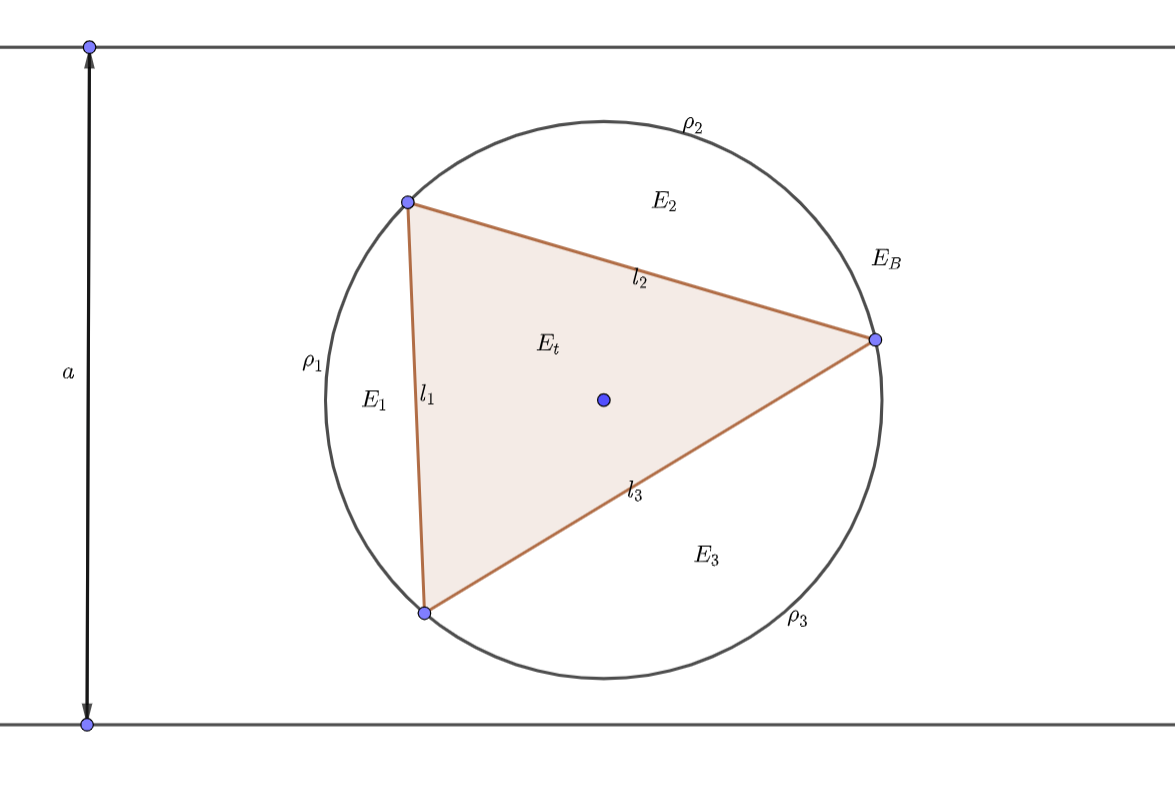
\includegraphics[width=0.8\textwidth]{figure.png}
}
% 表格模板
\renewcommand\arraystretch{0.8} % 设置表格高度为原来的0.8倍
\begin{table}[!htbp] % table标准
    \centering % 表格居中
    \begin{tabular}{p{1cm}<{\centering}p{1cm}<{\centering}p{3cm}<{\centering}p{5cm}<{\centering}} % 设置表格宽度
    %\begin{tabular}{cccc}
        \toprule
        $x_i$ & $f[x_1]$ & $f[x_i,x_{i+1}]$ & $f[x_i,x_{i+1},x_{i+2}]$ \\
        \midrule
        $x_0$ & $f(x_0)$ &                  &                          \\
        $x_0$ & $f(x_0)$ & $f'(x_0)$        &                          \\
        $x_0$ & $f(x_1)$ & $\frac{f(x_1)-f(x_0)}{x_1-x_0}$ & $\frac{f(x_1)-f(x_0)}{(x_1-x_0)^2}-\frac{f'(x_0)}{x_1-x_0}$\\
        \bottomrule
    \end{tabular}
\end{table}

\def\Log{\text{Log}} % 一个简单的宏定义
$\Log$ % 调用方法
\fi

\end{document}